\documentclass[twoside]{book}

% Packages required by doxygen
\usepackage{fixltx2e}
\usepackage{calc}
\usepackage{doxygen}
\usepackage[export]{adjustbox} % also loads graphicx
\usepackage{graphicx}
\usepackage[utf8]{inputenc}
\usepackage{makeidx}
\usepackage{multicol}
\usepackage{multirow}
\PassOptionsToPackage{warn}{textcomp}
\usepackage{textcomp}
\usepackage[nointegrals]{wasysym}
\usepackage[table]{xcolor}

% Font selection
\usepackage[T1]{fontenc}
\usepackage[scaled=.90]{helvet}
\usepackage{courier}
\usepackage{amssymb}
\usepackage{sectsty}
\renewcommand{\familydefault}{\sfdefault}
\allsectionsfont{%
  \fontseries{bc}\selectfont%
  \color{darkgray}%
}
\renewcommand{\DoxyLabelFont}{%
  \fontseries{bc}\selectfont%
  \color{darkgray}%
}
\newcommand{\+}{\discretionary{\mbox{\scriptsize$\hookleftarrow$}}{}{}}

% Page & text layout
\usepackage{geometry}
\geometry{%
  a4paper,%
  top=2.5cm,%
  bottom=2.5cm,%
  left=2.5cm,%
  right=2.5cm%
}
\tolerance=750
\hfuzz=15pt
\hbadness=750
\setlength{\emergencystretch}{15pt}
\setlength{\parindent}{0cm}
\setlength{\parskip}{3ex plus 2ex minus 2ex}
\makeatletter
\renewcommand{\paragraph}{%
  \@startsection{paragraph}{4}{0ex}{-1.0ex}{1.0ex}{%
    \normalfont\normalsize\bfseries\SS@parafont%
  }%
}
\renewcommand{\subparagraph}{%
  \@startsection{subparagraph}{5}{0ex}{-1.0ex}{1.0ex}{%
    \normalfont\normalsize\bfseries\SS@subparafont%
  }%
}
\makeatother

% Headers & footers
\usepackage{fancyhdr}
\pagestyle{fancyplain}
\fancyhead[LE]{\fancyplain{}{\bfseries\thepage}}
\fancyhead[CE]{\fancyplain{}{}}
\fancyhead[RE]{\fancyplain{}{\bfseries\leftmark}}
\fancyhead[LO]{\fancyplain{}{\bfseries\rightmark}}
\fancyhead[CO]{\fancyplain{}{}}
\fancyhead[RO]{\fancyplain{}{\bfseries\thepage}}
\fancyfoot[LE]{\fancyplain{}{}}
\fancyfoot[CE]{\fancyplain{}{}}
\fancyfoot[RE]{\fancyplain{}{\bfseries\scriptsize Generated by Doxygen }}
\fancyfoot[LO]{\fancyplain{}{\bfseries\scriptsize Generated by Doxygen }}
\fancyfoot[CO]{\fancyplain{}{}}
\fancyfoot[RO]{\fancyplain{}{}}
\renewcommand{\footrulewidth}{0.4pt}
\renewcommand{\chaptermark}[1]{%
  \markboth{#1}{}%
}
\renewcommand{\sectionmark}[1]{%
  \markright{\thesection\ #1}%
}

% Indices & bibliography
\usepackage{natbib}
\usepackage[titles]{tocloft}
\setcounter{tocdepth}{3}
\setcounter{secnumdepth}{5}
\makeindex

% Hyperlinks (required, but should be loaded last)
\usepackage{ifpdf}
\ifpdf
  \usepackage[pdftex,pagebackref=true]{hyperref}
\else
  \usepackage[ps2pdf,pagebackref=true]{hyperref}
\fi
\hypersetup{%
  colorlinks=true,%
  linkcolor=blue,%
  citecolor=blue,%
  unicode%
}

% Custom commands
\newcommand{\clearemptydoublepage}{%
  \newpage{\pagestyle{empty}\cleardoublepage}%
}

\usepackage{caption}
\captionsetup{labelsep=space,justification=centering,font={bf},singlelinecheck=off,skip=4pt,position=top}

%===== C O N T E N T S =====

\begin{document}

% Titlepage & ToC
\hypersetup{pageanchor=false,
             bookmarksnumbered=true,
             pdfencoding=unicode
            }
\pagenumbering{alph}
\begin{titlepage}
\vspace*{7cm}
\begin{center}%
{\Large Radix }\\
\vspace*{1cm}
{\large Generated by Doxygen 1.8.13}\\
\end{center}
\end{titlepage}
\clearemptydoublepage
\pagenumbering{roman}
\tableofcontents
\clearemptydoublepage
\pagenumbering{arabic}
\hypersetup{pageanchor=true}

%--- Begin generated contents ---
\chapter{Hierarchical Index}
\section{Class Hierarchy}
This inheritance list is sorted roughly, but not completely, alphabetically\+:\begin{DoxyCompactList}
\item \contentsline{section}{radix\+:\+:Equation\+Base}{\pageref{classradix_1_1EquationBase}}{}
\begin{DoxyCompactList}
\item \contentsline{section}{radix\+:\+:Equation}{\pageref{classradix_1_1Equation}}{}
\item \contentsline{section}{radix\+:\+:Function}{\pageref{classradix_1_1Function}}{}
\item \contentsline{section}{radix\+:\+:Value}{\pageref{classradix_1_1Value}}{}
\begin{DoxyCompactList}
\item \contentsline{section}{radix\+:\+:Long}{\pageref{classradix_1_1Long}}{}
\item \contentsline{section}{radix\+:\+:Variable}{\pageref{classradix_1_1Variable}}{}
\end{DoxyCompactList}
\end{DoxyCompactList}
\end{DoxyCompactList}

\chapter{Data Structure Index}
\section{Data Structures}
Here are the data structures with brief descriptions\+:\begin{DoxyCompactList}
\item\contentsline{section}{\hyperlink{classradix_1_1Equation}{radix\+::\+Equation} }{\pageref{classradix_1_1Equation}}{}
\item\contentsline{section}{\hyperlink{classradix_1_1EquationBase}{radix\+::\+Equation\+Base} }{\pageref{classradix_1_1EquationBase}}{}
\item\contentsline{section}{\hyperlink{classradix_1_1Function}{radix\+::\+Function} }{\pageref{classradix_1_1Function}}{}
\item\contentsline{section}{\hyperlink{classradix_1_1Long}{radix\+::\+Long} }{\pageref{classradix_1_1Long}}{}
\item\contentsline{section}{\hyperlink{classradix_1_1Value}{radix\+::\+Value} }{\pageref{classradix_1_1Value}}{}
\item\contentsline{section}{\hyperlink{classradix_1_1Variable}{radix\+::\+Variable} }{\pageref{classradix_1_1Variable}}{}
\end{DoxyCompactList}

\chapter{Data Structure Documentation}
\hypertarget{classradix_1_1Equation}{}\section{radix\+:\+:Equation Class Reference}
\label{classradix_1_1Equation}\index{radix\+::\+Equation@{radix\+::\+Equation}}
Inheritance diagram for radix\+:\+:Equation\+:\begin{figure}[H]
\begin{center}
\leavevmode
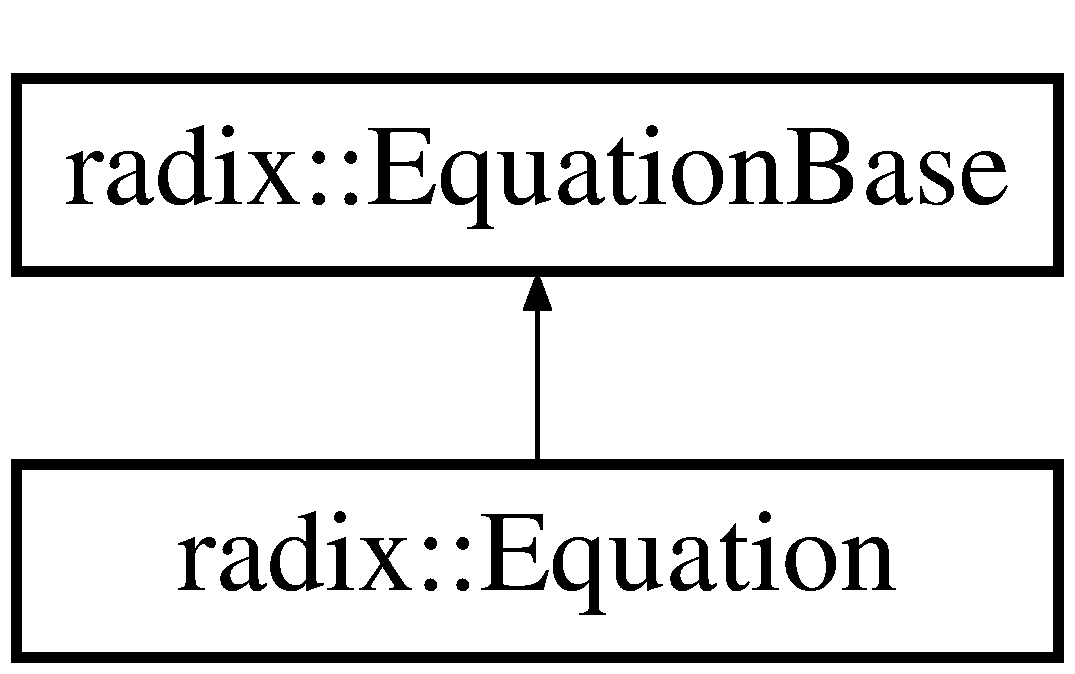
\includegraphics[height=2.000000cm]{classradix_1_1Equation}
\end{center}
\end{figure}
\subsection*{Public Types}
\begin{DoxyCompactItemize}
\item 
\mbox{\Hypertarget{classradix_1_1Equation_af14b805e134e0b97985269ded61a0ff3}\label{classradix_1_1Equation_af14b805e134e0b97985269ded61a0ff3}} 
typedef std\+::vector$<$ std\+::shared\+\_\+ptr$<$ \hyperlink{classradix_1_1EquationBase}{Equation\+Base} $>$ $>$\+::reference {\bfseries reference}
\item 
\mbox{\Hypertarget{classradix_1_1Equation_a27b9024e87f9fc6fdc69d9acfb169c13}\label{classradix_1_1Equation_a27b9024e87f9fc6fdc69d9acfb169c13}} 
typedef std\+::vector$<$ std\+::shared\+\_\+ptr$<$ \hyperlink{classradix_1_1EquationBase}{Equation\+Base} $>$ $>$\+::const\+\_\+reference {\bfseries const\+\_\+reference}
\item 
\mbox{\Hypertarget{classradix_1_1Equation_acbf3eb05aca712c25798ee3906167649}\label{classradix_1_1Equation_acbf3eb05aca712c25798ee3906167649}} 
typedef std\+::vector$<$ std\+::shared\+\_\+ptr$<$ \hyperlink{classradix_1_1EquationBase}{Equation\+Base} $>$ $>$\+::pointer {\bfseries pointer}
\item 
\mbox{\Hypertarget{classradix_1_1Equation_aa6ad9cd7762a256ffcbfb666dd81b869}\label{classradix_1_1Equation_aa6ad9cd7762a256ffcbfb666dd81b869}} 
typedef std\+::vector$<$ std\+::shared\+\_\+ptr$<$ \hyperlink{classradix_1_1EquationBase}{Equation\+Base} $>$ $>$\+::const\+\_\+pointer {\bfseries const\+\_\+pointer}
\item 
\mbox{\Hypertarget{classradix_1_1Equation_a3010f04d61440cb48f96fa8a04847f77}\label{classradix_1_1Equation_a3010f04d61440cb48f96fa8a04847f77}} 
typedef std\+::vector$<$ std\+::shared\+\_\+ptr$<$ \hyperlink{classradix_1_1EquationBase}{Equation\+Base} $>$ $>$\+::iterator {\bfseries iterator}
\item 
\mbox{\Hypertarget{classradix_1_1Equation_ad5b7cb4508fc13c9a9a9e019a5f883b5}\label{classradix_1_1Equation_ad5b7cb4508fc13c9a9a9e019a5f883b5}} 
typedef std\+::vector$<$ std\+::shared\+\_\+ptr$<$ \hyperlink{classradix_1_1EquationBase}{Equation\+Base} $>$ $>$\+::const\+\_\+iterator {\bfseries const\+\_\+iterator}
\item 
\mbox{\Hypertarget{classradix_1_1Equation_aafcd464f7492c0f0483b1c2e66893138}\label{classradix_1_1Equation_aafcd464f7492c0f0483b1c2e66893138}} 
typedef std\+::vector$<$ std\+::shared\+\_\+ptr$<$ \hyperlink{classradix_1_1EquationBase}{Equation\+Base} $>$ $>$\+::reverse\+\_\+iterator {\bfseries reverse\+\_\+iterator}
\item 
\mbox{\Hypertarget{classradix_1_1Equation_a3641db32538ca872e1cd874d533dcbdd}\label{classradix_1_1Equation_a3641db32538ca872e1cd874d533dcbdd}} 
typedef std\+::vector$<$ std\+::shared\+\_\+ptr$<$ \hyperlink{classradix_1_1EquationBase}{Equation\+Base} $>$ $>$\+::const\+\_\+reverse\+\_\+iterator {\bfseries const\+\_\+reverse\+\_\+iterator}
\end{DoxyCompactItemize}
\subsection*{Public Member Functions}
\begin{DoxyCompactItemize}
\item 
\mbox{\Hypertarget{classradix_1_1Equation_a3fce338abc1152dd32c9d91be064847a}\label{classradix_1_1Equation_a3fce338abc1152dd32c9d91be064847a}} 
reference {\bfseries front} ()
\item 
\mbox{\Hypertarget{classradix_1_1Equation_afcfe55da13a33f91a6d144337319659a}\label{classradix_1_1Equation_afcfe55da13a33f91a6d144337319659a}} 
const\+\_\+reference {\bfseries front} () const
\item 
\mbox{\Hypertarget{classradix_1_1Equation_aa1206fe0f6caaf9a47fee7e57c66c0e9}\label{classradix_1_1Equation_aa1206fe0f6caaf9a47fee7e57c66c0e9}} 
const\+\_\+reference {\bfseries cfront} () const
\item 
\mbox{\Hypertarget{classradix_1_1Equation_af282cd564c82981448bc0fcdc9b056cc}\label{classradix_1_1Equation_af282cd564c82981448bc0fcdc9b056cc}} 
reference {\bfseries back} ()
\item 
\mbox{\Hypertarget{classradix_1_1Equation_a5f5da71f14a54b605d17a39aa4b539a6}\label{classradix_1_1Equation_a5f5da71f14a54b605d17a39aa4b539a6}} 
const\+\_\+reference {\bfseries back} () const
\item 
\mbox{\Hypertarget{classradix_1_1Equation_ae39cec445f3dc63cb1aadd2e5bcf9c8e}\label{classradix_1_1Equation_ae39cec445f3dc63cb1aadd2e5bcf9c8e}} 
const\+\_\+reference {\bfseries cback} () const
\item 
\mbox{\Hypertarget{classradix_1_1Equation_a8969ede3db3237d74b893beb2a3ad516}\label{classradix_1_1Equation_a8969ede3db3237d74b893beb2a3ad516}} 
iterator {\bfseries begin} ()
\item 
\mbox{\Hypertarget{classradix_1_1Equation_a26e3c7e211b1290ac5a5ad4633594c99}\label{classradix_1_1Equation_a26e3c7e211b1290ac5a5ad4633594c99}} 
const\+\_\+iterator {\bfseries begin} () const
\item 
\mbox{\Hypertarget{classradix_1_1Equation_ad700ce46a4e31c3fd91144711ab372be}\label{classradix_1_1Equation_ad700ce46a4e31c3fd91144711ab372be}} 
const\+\_\+iterator {\bfseries cbegin} () const
\item 
\mbox{\Hypertarget{classradix_1_1Equation_aafd68b8b541b17af7fa7bbe54620aa1a}\label{classradix_1_1Equation_aafd68b8b541b17af7fa7bbe54620aa1a}} 
iterator {\bfseries end} ()
\item 
\mbox{\Hypertarget{classradix_1_1Equation_a3bc3acdc2cc562af75486cb27128e891}\label{classradix_1_1Equation_a3bc3acdc2cc562af75486cb27128e891}} 
const\+\_\+iterator {\bfseries end} () const
\item 
\mbox{\Hypertarget{classradix_1_1Equation_a853a4cbb48e60e58d55f0f1e6bca607b}\label{classradix_1_1Equation_a853a4cbb48e60e58d55f0f1e6bca607b}} 
const\+\_\+iterator {\bfseries cend} () const
\item 
\mbox{\Hypertarget{classradix_1_1Equation_a424dc6c48c89e153c9f298e28f42b2c7}\label{classradix_1_1Equation_a424dc6c48c89e153c9f298e28f42b2c7}} 
reverse\+\_\+iterator {\bfseries rbegin} ()
\item 
\mbox{\Hypertarget{classradix_1_1Equation_a4ed8311ef1a74bedf12cecb59a74c94e}\label{classradix_1_1Equation_a4ed8311ef1a74bedf12cecb59a74c94e}} 
const\+\_\+reverse\+\_\+iterator {\bfseries rbegin} () const
\item 
\mbox{\Hypertarget{classradix_1_1Equation_a3ea3b6c4b675fc243a09e703cacdb68d}\label{classradix_1_1Equation_a3ea3b6c4b675fc243a09e703cacdb68d}} 
const\+\_\+reverse\+\_\+iterator {\bfseries crbegin} () const
\item 
\mbox{\Hypertarget{classradix_1_1Equation_a59bbd6b42ff166f0624dc922dbeaad95}\label{classradix_1_1Equation_a59bbd6b42ff166f0624dc922dbeaad95}} 
reverse\+\_\+iterator {\bfseries rend} ()
\item 
\mbox{\Hypertarget{classradix_1_1Equation_a405c72740924311f647b9f45e30b40c7}\label{classradix_1_1Equation_a405c72740924311f647b9f45e30b40c7}} 
const\+\_\+reverse\+\_\+iterator {\bfseries rend} () const
\item 
\mbox{\Hypertarget{classradix_1_1Equation_a94ab3f3fda0dc831b0805af67ec97604}\label{classradix_1_1Equation_a94ab3f3fda0dc831b0805af67ec97604}} 
const\+\_\+reverse\+\_\+iterator {\bfseries crend} () const
\item 
\mbox{\Hypertarget{classradix_1_1Equation_ad54cf2410ccc309578327da863f8845c}\label{classradix_1_1Equation_ad54cf2410ccc309578327da863f8845c}} 
void {\bfseries clear} ()
\item 
\mbox{\Hypertarget{classradix_1_1Equation_a32363cf88af0d74043904d4c67d0f358}\label{classradix_1_1Equation_a32363cf88af0d74043904d4c67d0f358}} 
void {\bfseries insert} (const\+\_\+iterator pos, const std\+::shared\+\_\+ptr$<$ \hyperlink{classradix_1_1EquationBase}{Equation\+Base} $>$ \&val)
\item 
\mbox{\Hypertarget{classradix_1_1Equation_a897f1dc523e017bf5d01d5f0db3cb7c5}\label{classradix_1_1Equation_a897f1dc523e017bf5d01d5f0db3cb7c5}} 
void {\bfseries erase} (const\+\_\+iterator pos)
\item 
\mbox{\Hypertarget{classradix_1_1Equation_a47f65d0d976760f41e75a3b2ce084c94}\label{classradix_1_1Equation_a47f65d0d976760f41e75a3b2ce084c94}} 
void {\bfseries erase} (const\+\_\+iterator first, const\+\_\+iterator last)
\item 
\mbox{\Hypertarget{classradix_1_1Equation_ada8ce44d7f5d9e82613b16e0e1023629}\label{classradix_1_1Equation_ada8ce44d7f5d9e82613b16e0e1023629}} 
void {\bfseries push\+\_\+back} (const std\+::shared\+\_\+ptr$<$ \hyperlink{classradix_1_1EquationBase}{Equation\+Base} $>$ \&val)
\item 
\mbox{\Hypertarget{classradix_1_1Equation_a7657e48a6520c21e15cd4e52a6261bca}\label{classradix_1_1Equation_a7657e48a6520c21e15cd4e52a6261bca}} 
void {\bfseries pop\+\_\+back} ()
\item 
\mbox{\Hypertarget{classradix_1_1Equation_ab07495c0e6420d7063d0133849743c4f}\label{classradix_1_1Equation_ab07495c0e6420d7063d0133849743c4f}} 
virtual std\+::string {\bfseries Latex} () const
\end{DoxyCompactItemize}
\subsection*{Additional Inherited Members}


The documentation for this class was generated from the following files\+:\begin{DoxyCompactItemize}
\item 
include/equation/equation.\+hpp\item 
source/equation/equation.\+cpp\end{DoxyCompactItemize}

\hypertarget{classradix_1_1EquationBase}{}\section{radix\+:\+:Equation\+Base Class Reference}
\label{classradix_1_1EquationBase}\index{radix\+::\+Equation\+Base@{radix\+::\+Equation\+Base}}
Inheritance diagram for radix\+:\+:Equation\+Base\+:\begin{figure}[H]
\begin{center}
\leavevmode
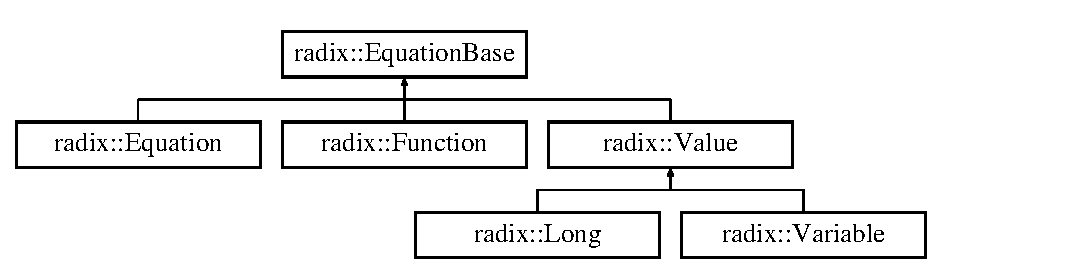
\includegraphics[height=3.000000cm]{classradix_1_1EquationBase}
\end{center}
\end{figure}
\subsection*{Public Member Functions}
\begin{DoxyCompactItemize}
\item 
\mbox{\Hypertarget{classradix_1_1EquationBase_a88482ba80ce76c683abae39cab450b1b}\label{classradix_1_1EquationBase_a88482ba80ce76c683abae39cab450b1b}} 
{\bfseries Equation\+Base} (const Equation\+Type \&type)
\item 
\mbox{\Hypertarget{classradix_1_1EquationBase_ae251a2185ff420ad61eeb7444bb26e02}\label{classradix_1_1EquationBase_ae251a2185ff420ad61eeb7444bb26e02}} 
virtual std\+::string {\bfseries Latex} () const
\end{DoxyCompactItemize}
\subsection*{Data Fields}
\begin{DoxyCompactItemize}
\item 
\mbox{\Hypertarget{classradix_1_1EquationBase_a558f49069025e281b98abd8560c80090}\label{classradix_1_1EquationBase_a558f49069025e281b98abd8560c80090}} 
Equation\+Type {\bfseries type\+\_\+}
\end{DoxyCompactItemize}


The documentation for this class was generated from the following files\+:\begin{DoxyCompactItemize}
\item 
include/equation\+\_\+base.\+hpp\item 
source/equation\+\_\+base.\+cpp\end{DoxyCompactItemize}

\hypertarget{classradix_1_1Function}{}\section{radix\+:\+:Function Class Reference}
\label{classradix_1_1Function}\index{radix\+::\+Function@{radix\+::\+Function}}
Inheritance diagram for radix\+:\+:Function\+:\begin{figure}[H]
\begin{center}
\leavevmode
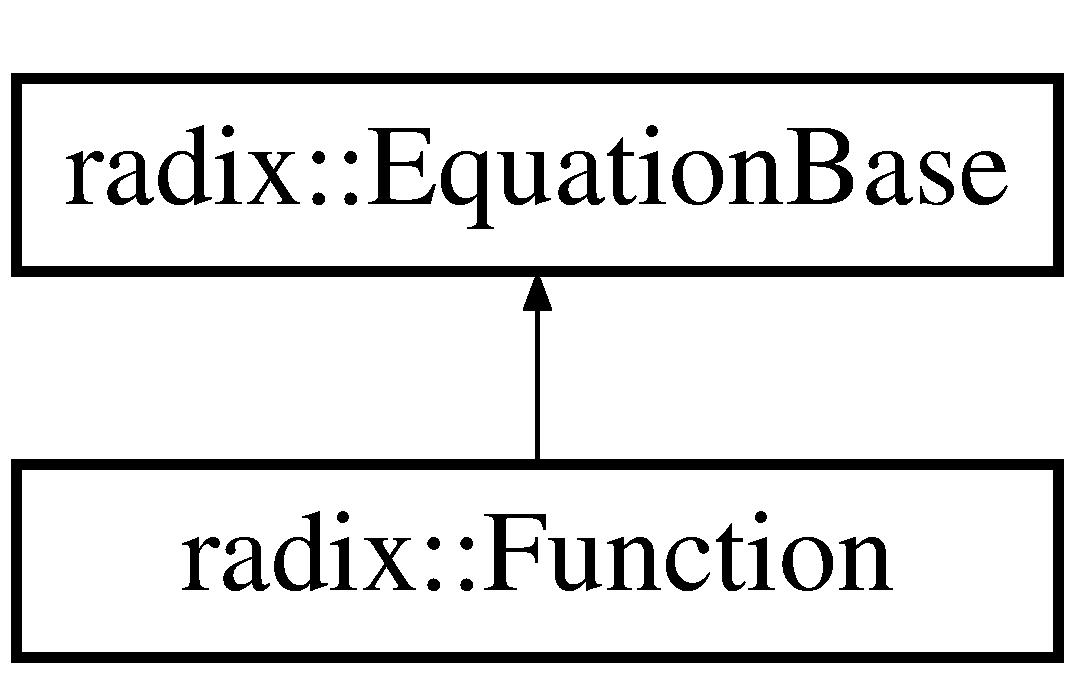
\includegraphics[height=2.000000cm]{classradix_1_1Function}
\end{center}
\end{figure}
\subsection*{Public Member Functions}
\begin{DoxyCompactItemize}
\item 
\mbox{\Hypertarget{classradix_1_1Function_a3d03267593beba87b9b1064065cdac60}\label{classradix_1_1Function_a3d03267593beba87b9b1064065cdac60}} 
{\bfseries Function} (std\+::size\+\_\+t n\+\_\+args, std\+::size\+\_\+t n\+\_\+default)
\item 
\mbox{\Hypertarget{classradix_1_1Function_a341d93b270c5c539a6dadc1bd7bbd3f0}\label{classradix_1_1Function_a341d93b270c5c539a6dadc1bd7bbd3f0}} 
{\footnotesize template$<$typename... Args$>$ }\\void {\bfseries operator()} (const Args \&... args)
\end{DoxyCompactItemize}
\subsection*{Additional Inherited Members}


The documentation for this class was generated from the following files\+:\begin{DoxyCompactItemize}
\item 
include/function/function.\+hpp\item 
source/function/function.\+cpp\end{DoxyCompactItemize}

\hypertarget{classradix_1_1Long}{}\section{radix\+:\+:Long Class Reference}
\label{classradix_1_1Long}\index{radix\+::\+Long@{radix\+::\+Long}}
Inheritance diagram for radix\+:\+:Long\+:\begin{figure}[H]
\begin{center}
\leavevmode
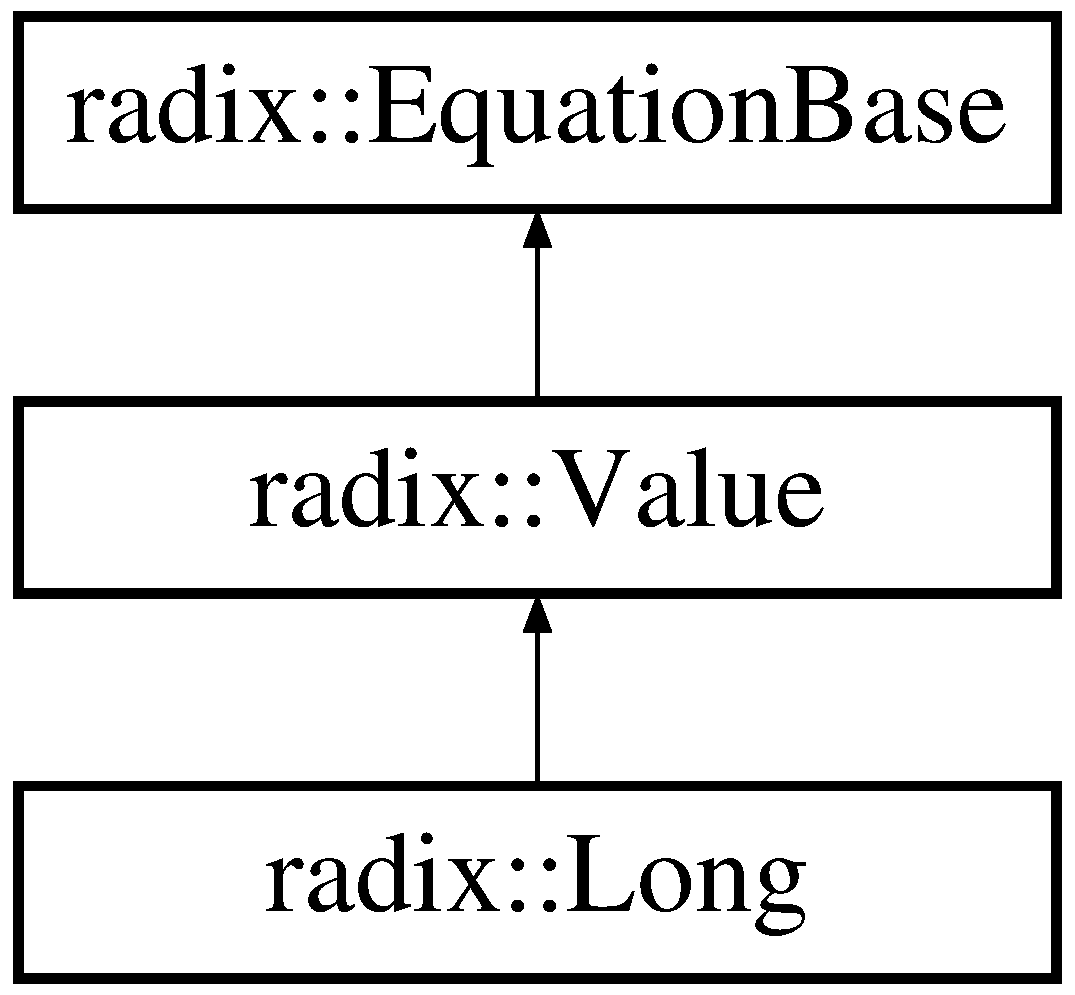
\includegraphics[height=3.000000cm]{classradix_1_1Long}
\end{center}
\end{figure}
\subsection*{Public Member Functions}
\begin{DoxyCompactItemize}
\item 
\mbox{\Hypertarget{classradix_1_1Long_af07721c946aaa24cd0ad0de31c3ca3f3}\label{classradix_1_1Long_af07721c946aaa24cd0ad0de31c3ca3f3}} 
{\bfseries Long} (int val)
\item 
\mbox{\Hypertarget{classradix_1_1Long_acac6ededfc5c4018175951b715a583df}\label{classradix_1_1Long_acac6ededfc5c4018175951b715a583df}} 
{\bfseries Long} (long int val)
\item 
\mbox{\Hypertarget{classradix_1_1Long_a698b95031b0899c044926d0c0f1f1703}\label{classradix_1_1Long_a698b95031b0899c044926d0c0f1f1703}} 
{\bfseries Long} (long long int val)
\item 
\mbox{\Hypertarget{classradix_1_1Long_a1ef9ea8476ae4e6c629d1cd790603619}\label{classradix_1_1Long_a1ef9ea8476ae4e6c629d1cd790603619}} 
{\bfseries Long} (unsigned int val)
\item 
\mbox{\Hypertarget{classradix_1_1Long_aff3bca9e174962b47124df0249439850}\label{classradix_1_1Long_aff3bca9e174962b47124df0249439850}} 
{\bfseries Long} (unsigned long int val)
\item 
\mbox{\Hypertarget{classradix_1_1Long_af5cdaf8c62a5e4074a4a07a305c4960a}\label{classradix_1_1Long_af5cdaf8c62a5e4074a4a07a305c4960a}} 
{\bfseries Long} (unsigned long long int val)
\item 
\mbox{\Hypertarget{classradix_1_1Long_a6bf8d93ea07aa0a5ab24d355de59fbe1}\label{classradix_1_1Long_a6bf8d93ea07aa0a5ab24d355de59fbe1}} 
{\bfseries Long} (float val)
\item 
\mbox{\Hypertarget{classradix_1_1Long_a734b57ccc1afa1996b710c9b3e01495f}\label{classradix_1_1Long_a734b57ccc1afa1996b710c9b3e01495f}} 
{\bfseries Long} (double val)
\item 
\mbox{\Hypertarget{classradix_1_1Long_a71dc131ba394fd831442af0571cea6b6}\label{classradix_1_1Long_a71dc131ba394fd831442af0571cea6b6}} 
{\bfseries Long} (long double val)
\item 
\mbox{\Hypertarget{classradix_1_1Long_a5cb8e4b96d292631c8af62195ecfb784}\label{classradix_1_1Long_a5cb8e4b96d292631c8af62195ecfb784}} 
{\bfseries Long} (std\+::string val)
\item 
\mbox{\Hypertarget{classradix_1_1Long_acaa8b35cf83b7595aa33856ba88b19ea}\label{classradix_1_1Long_acaa8b35cf83b7595aa33856ba88b19ea}} 
{\bfseries Long} (const char $\ast$val)
\item 
\mbox{\Hypertarget{classradix_1_1Long_a0d938a279b3973c1df096b1a242c4294}\label{classradix_1_1Long_a0d938a279b3973c1df096b1a242c4294}} 
{\bfseries Long} (int val, std\+::size\+\_\+t prec)
\item 
\mbox{\Hypertarget{classradix_1_1Long_af02fcb04d4e31810dfd96197c1aabbb7}\label{classradix_1_1Long_af02fcb04d4e31810dfd96197c1aabbb7}} 
{\bfseries Long} (long int val, std\+::size\+\_\+t prec)
\item 
\mbox{\Hypertarget{classradix_1_1Long_a1172cd96885db3bc64b7c176b9d19188}\label{classradix_1_1Long_a1172cd96885db3bc64b7c176b9d19188}} 
{\bfseries Long} (long long int val, std\+::size\+\_\+t prec)
\item 
\mbox{\Hypertarget{classradix_1_1Long_af271dfca36d5e06525b01947f70ed0e2}\label{classradix_1_1Long_af271dfca36d5e06525b01947f70ed0e2}} 
{\bfseries Long} (unsigned int val, std\+::size\+\_\+t prec)
\item 
\mbox{\Hypertarget{classradix_1_1Long_ae6bf7d79dd34fcb24d90fbac12fde53d}\label{classradix_1_1Long_ae6bf7d79dd34fcb24d90fbac12fde53d}} 
{\bfseries Long} (unsigned long int val, std\+::size\+\_\+t prec)
\item 
\mbox{\Hypertarget{classradix_1_1Long_a66e89240bd4f7c4690bff7f4943f97e4}\label{classradix_1_1Long_a66e89240bd4f7c4690bff7f4943f97e4}} 
{\bfseries Long} (unsigned long long int val, std\+::size\+\_\+t prec)
\item 
\mbox{\Hypertarget{classradix_1_1Long_a1c3f9b2ad843c4bf66bf602f12ce300d}\label{classradix_1_1Long_a1c3f9b2ad843c4bf66bf602f12ce300d}} 
{\bfseries Long} (float val, std\+::size\+\_\+t prec)
\item 
\mbox{\Hypertarget{classradix_1_1Long_ae94f450a01a686857b587f46ff02cd69}\label{classradix_1_1Long_ae94f450a01a686857b587f46ff02cd69}} 
{\bfseries Long} (double val, std\+::size\+\_\+t prec)
\item 
\mbox{\Hypertarget{classradix_1_1Long_abaa677963a90987b2bef8c645b7d6d47}\label{classradix_1_1Long_abaa677963a90987b2bef8c645b7d6d47}} 
{\bfseries Long} (long double val, std\+::size\+\_\+t prec)
\item 
\mbox{\Hypertarget{classradix_1_1Long_a03c37ee6515eb03e2251fb6f318c22bf}\label{classradix_1_1Long_a03c37ee6515eb03e2251fb6f318c22bf}} 
{\bfseries Long} (std\+::string val, std\+::size\+\_\+t prec)
\item 
\mbox{\Hypertarget{classradix_1_1Long_a88c8a6361a9cd3c6dbbf88128b98ea42}\label{classradix_1_1Long_a88c8a6361a9cd3c6dbbf88128b98ea42}} 
{\bfseries Long} (const char $\ast$val, std\+::size\+\_\+t prec)
\item 
\mbox{\Hypertarget{classradix_1_1Long_a715bd827d23c82ab8eedc962a19322ef}\label{classradix_1_1Long_a715bd827d23c82ab8eedc962a19322ef}} 
{\bfseries Long} (const \hyperlink{classradix_1_1Long}{Long} \&copy)
\item 
\mbox{\Hypertarget{classradix_1_1Long_a7cd2677afe432d015b92a24160920271}\label{classradix_1_1Long_a7cd2677afe432d015b92a24160920271}} 
void {\bfseries Set} (int val)
\item 
\mbox{\Hypertarget{classradix_1_1Long_a7f5b39276793bfc69f9524b4af04f412}\label{classradix_1_1Long_a7f5b39276793bfc69f9524b4af04f412}} 
void {\bfseries Set} (long int val)
\item 
\mbox{\Hypertarget{classradix_1_1Long_a648d55ccfdfe8d1b623a0fbc9896c873}\label{classradix_1_1Long_a648d55ccfdfe8d1b623a0fbc9896c873}} 
void {\bfseries Set} (long long int val)
\item 
\mbox{\Hypertarget{classradix_1_1Long_abf68908f3fdea6de02dc51b91d9a462f}\label{classradix_1_1Long_abf68908f3fdea6de02dc51b91d9a462f}} 
void {\bfseries Set} (unsigned int val)
\item 
\mbox{\Hypertarget{classradix_1_1Long_a4de494937db63611d0f57544e2945837}\label{classradix_1_1Long_a4de494937db63611d0f57544e2945837}} 
void {\bfseries Set} (unsigned long int val)
\item 
\mbox{\Hypertarget{classradix_1_1Long_ad4a31314efe4bbe22c7db1547fd296f4}\label{classradix_1_1Long_ad4a31314efe4bbe22c7db1547fd296f4}} 
void {\bfseries Set} (unsigned long long int val)
\item 
\mbox{\Hypertarget{classradix_1_1Long_a6b7b0e36c63671fd7823830e4b0f7d0f}\label{classradix_1_1Long_a6b7b0e36c63671fd7823830e4b0f7d0f}} 
void {\bfseries Set} (float val)
\item 
\mbox{\Hypertarget{classradix_1_1Long_ab873afac8e394d0e881bef36f8cfc0a2}\label{classradix_1_1Long_ab873afac8e394d0e881bef36f8cfc0a2}} 
void {\bfseries Set} (double val)
\item 
\mbox{\Hypertarget{classradix_1_1Long_a50a28cf7e673f5053d3600dbe2d03f91}\label{classradix_1_1Long_a50a28cf7e673f5053d3600dbe2d03f91}} 
void {\bfseries Set} (long double val)
\item 
\mbox{\Hypertarget{classradix_1_1Long_a49fdefee26b1cb83105b882de678b924}\label{classradix_1_1Long_a49fdefee26b1cb83105b882de678b924}} 
void {\bfseries Set} (std\+::string val)
\item 
\mbox{\Hypertarget{classradix_1_1Long_a999ce44f23502b9b0c88a93af68bf8d4}\label{classradix_1_1Long_a999ce44f23502b9b0c88a93af68bf8d4}} 
void {\bfseries Set} (const char $\ast$val)
\item 
\mbox{\Hypertarget{classradix_1_1Long_a24830514ccb8e24e8db8dbf6b9712f5e}\label{classradix_1_1Long_a24830514ccb8e24e8db8dbf6b9712f5e}} 
void {\bfseries Set} (const \hyperlink{classradix_1_1Long}{Long} \&copy)
\item 
\mbox{\Hypertarget{classradix_1_1Long_ab948f973d129d3e8b592efd0db502326}\label{classradix_1_1Long_ab948f973d129d3e8b592efd0db502326}} 
void {\bfseries Data} (mpfr\+\_\+t \&val) const
\item 
\mbox{\Hypertarget{classradix_1_1Long_af675e7bbffadb7cb8b5c53f70ac65f22}\label{classradix_1_1Long_af675e7bbffadb7cb8b5c53f70ac65f22}} 
std\+::size\+\_\+t {\bfseries Get\+Precision} () const
\item 
\mbox{\Hypertarget{classradix_1_1Long_a0fc977c188e5a7fd78e82290d266b60a}\label{classradix_1_1Long_a0fc977c188e5a7fd78e82290d266b60a}} 
void {\bfseries Set\+Precision} (std\+::size\+\_\+t bits)
\item 
\mbox{\Hypertarget{classradix_1_1Long_a59f6736ef10308cc24379d32a38d4adb}\label{classradix_1_1Long_a59f6736ef10308cc24379d32a38d4adb}} 
std\+::string {\bfseries Get\+String} (int prec=-\/1, bool left=false) const
\item 
\mbox{\Hypertarget{classradix_1_1Long_a6a1ac9d31d581b9d448595dfa0c4cb2b}\label{classradix_1_1Long_a6a1ac9d31d581b9d448595dfa0c4cb2b}} 
virtual std\+::string {\bfseries Latex} () const
\item 
\mbox{\Hypertarget{classradix_1_1Long_ad99cd1f4544f64a507ea5b8d7d3debc4}\label{classradix_1_1Long_ad99cd1f4544f64a507ea5b8d7d3debc4}} 
\hyperlink{classradix_1_1Long}{Long} \& {\bfseries operator=} (int val)
\item 
\mbox{\Hypertarget{classradix_1_1Long_af9ec8fca0048e12e980a58e75ac79a9d}\label{classradix_1_1Long_af9ec8fca0048e12e980a58e75ac79a9d}} 
\hyperlink{classradix_1_1Long}{Long} \& {\bfseries operator=} (long int val)
\item 
\mbox{\Hypertarget{classradix_1_1Long_a0d099f53a1f660ede70682a5694c22cd}\label{classradix_1_1Long_a0d099f53a1f660ede70682a5694c22cd}} 
\hyperlink{classradix_1_1Long}{Long} \& {\bfseries operator=} (long long int val)
\item 
\mbox{\Hypertarget{classradix_1_1Long_ac7df3c49fee561843da1825529c50729}\label{classradix_1_1Long_ac7df3c49fee561843da1825529c50729}} 
\hyperlink{classradix_1_1Long}{Long} \& {\bfseries operator=} (unsigned int val)
\item 
\mbox{\Hypertarget{classradix_1_1Long_ad809ddec119b8813f92e84f532857f83}\label{classradix_1_1Long_ad809ddec119b8813f92e84f532857f83}} 
\hyperlink{classradix_1_1Long}{Long} \& {\bfseries operator=} (unsigned long int val)
\item 
\mbox{\Hypertarget{classradix_1_1Long_a20c03d141ec3b80c36d1552066e451d7}\label{classradix_1_1Long_a20c03d141ec3b80c36d1552066e451d7}} 
\hyperlink{classradix_1_1Long}{Long} \& {\bfseries operator=} (unsigned long long int val)
\item 
\mbox{\Hypertarget{classradix_1_1Long_a6371a1695ef4d786992a02afd71c9e39}\label{classradix_1_1Long_a6371a1695ef4d786992a02afd71c9e39}} 
\hyperlink{classradix_1_1Long}{Long} \& {\bfseries operator=} (float val)
\item 
\mbox{\Hypertarget{classradix_1_1Long_a16dd9c1a39d650de0e1cf3b2636f8fdd}\label{classradix_1_1Long_a16dd9c1a39d650de0e1cf3b2636f8fdd}} 
\hyperlink{classradix_1_1Long}{Long} \& {\bfseries operator=} (double val)
\item 
\mbox{\Hypertarget{classradix_1_1Long_a87d32e61a119f0a05f28245bbf8a1cfc}\label{classradix_1_1Long_a87d32e61a119f0a05f28245bbf8a1cfc}} 
\hyperlink{classradix_1_1Long}{Long} \& {\bfseries operator=} (long double val)
\item 
\mbox{\Hypertarget{classradix_1_1Long_a63fe9e2b3670e2914b73639afca8fa42}\label{classradix_1_1Long_a63fe9e2b3670e2914b73639afca8fa42}} 
\hyperlink{classradix_1_1Long}{Long} \& {\bfseries operator=} (std\+::string val)
\item 
\mbox{\Hypertarget{classradix_1_1Long_a842758eda77e6e2d4f1ca6c1fcff6684}\label{classradix_1_1Long_a842758eda77e6e2d4f1ca6c1fcff6684}} 
\hyperlink{classradix_1_1Long}{Long} \& {\bfseries operator=} (const char $\ast$val)
\item 
\mbox{\Hypertarget{classradix_1_1Long_acde06629cdae07ab558f338aa9c9624f}\label{classradix_1_1Long_acde06629cdae07ab558f338aa9c9624f}} 
\hyperlink{classradix_1_1Long}{Long} \& {\bfseries operator=} (const \hyperlink{classradix_1_1Long}{Long} \&val)
\item 
\mbox{\Hypertarget{classradix_1_1Long_a666fd63de5da779999097866422554e4}\label{classradix_1_1Long_a666fd63de5da779999097866422554e4}} 
\hyperlink{classradix_1_1Long}{Long} \& {\bfseries operator+=} (const \hyperlink{classradix_1_1Long}{Long} \&rhs)
\item 
\mbox{\Hypertarget{classradix_1_1Long_abb38162f1cb185af3b756cf8126cf921}\label{classradix_1_1Long_abb38162f1cb185af3b756cf8126cf921}} 
\hyperlink{classradix_1_1Long}{Long} \& {\bfseries operator-\/=} (const \hyperlink{classradix_1_1Long}{Long} \&rhs)
\item 
\mbox{\Hypertarget{classradix_1_1Long_a8d320bc31548b5d44272e8cf04464c62}\label{classradix_1_1Long_a8d320bc31548b5d44272e8cf04464c62}} 
\hyperlink{classradix_1_1Long}{Long} \& {\bfseries operator$\ast$=} (const \hyperlink{classradix_1_1Long}{Long} \&rhs)
\item 
\mbox{\Hypertarget{classradix_1_1Long_a386f2a61d8a37797160bcb9868af9ffe}\label{classradix_1_1Long_a386f2a61d8a37797160bcb9868af9ffe}} 
\hyperlink{classradix_1_1Long}{Long} \& {\bfseries operator/=} (const \hyperlink{classradix_1_1Long}{Long} \&rhs)
\item 
\mbox{\Hypertarget{classradix_1_1Long_a227a6f77719c6f7a5c45c0c38a782f2e}\label{classradix_1_1Long_a227a6f77719c6f7a5c45c0c38a782f2e}} 
{\bfseries operator std\+::shared\+\_\+ptr$<$ Value $>$} ()
\item 
\mbox{\Hypertarget{classradix_1_1Long_a6ee622b45931bffaf8729e1d8b9c344a}\label{classradix_1_1Long_a6ee622b45931bffaf8729e1d8b9c344a}} 
{\bfseries operator std\+::shared\+\_\+ptr$<$ Equation\+Base $>$} ()
\end{DoxyCompactItemize}
\subsection*{Data Fields}
\begin{DoxyCompactItemize}
\item 
\mbox{\Hypertarget{classradix_1_1Long_a5c1262411dd23a7b9c0e6b8e064b7f58}\label{classradix_1_1Long_a5c1262411dd23a7b9c0e6b8e064b7f58}} 
mpfr\+\_\+t {\bfseries value\+\_\+}
\end{DoxyCompactItemize}


The documentation for this class was generated from the following files\+:\begin{DoxyCompactItemize}
\item 
include/value/long.\+hpp\item 
source/value/long.\+cpp\end{DoxyCompactItemize}

\hypertarget{classradix_1_1Value}{}\section{radix\+:\+:Value Class Reference}
\label{classradix_1_1Value}\index{radix\+::\+Value@{radix\+::\+Value}}
Inheritance diagram for radix\+:\+:Value\+:\begin{figure}[H]
\begin{center}
\leavevmode
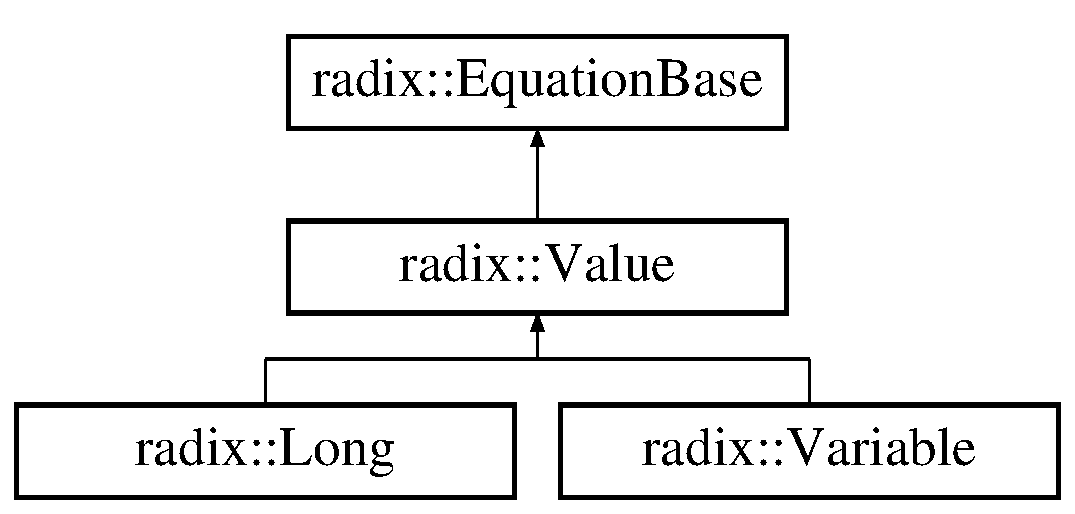
\includegraphics[height=3.000000cm]{classradix_1_1Value}
\end{center}
\end{figure}
\subsection*{Public Member Functions}
\begin{DoxyCompactItemize}
\item 
\mbox{\Hypertarget{classradix_1_1Value_abe99ba991c4009aca8ab9a775d461a11}\label{classradix_1_1Value_abe99ba991c4009aca8ab9a775d461a11}} 
{\bfseries Value} (Value\+Type type)
\item 
\mbox{\Hypertarget{classradix_1_1Value_a2eac6c73b8e2a8131407bca685b05299}\label{classradix_1_1Value_a2eac6c73b8e2a8131407bca685b05299}} 
virtual std\+::string {\bfseries Latex} () const
\end{DoxyCompactItemize}
\subsection*{Data Fields}
\begin{DoxyCompactItemize}
\item 
\mbox{\Hypertarget{classradix_1_1Value_a5f6d52b7c39af605d22e7af2b777e045}\label{classradix_1_1Value_a5f6d52b7c39af605d22e7af2b777e045}} 
Value\+Type {\bfseries type\+\_\+}
\end{DoxyCompactItemize}


The documentation for this class was generated from the following files\+:\begin{DoxyCompactItemize}
\item 
include/value/value.\+hpp\item 
source/value/value.\+cpp\end{DoxyCompactItemize}

\hypertarget{classradix_1_1Variable}{}\section{radix\+:\+:Variable Class Reference}
\label{classradix_1_1Variable}\index{radix\+::\+Variable@{radix\+::\+Variable}}
Inheritance diagram for radix\+:\+:Variable\+:\begin{figure}[H]
\begin{center}
\leavevmode
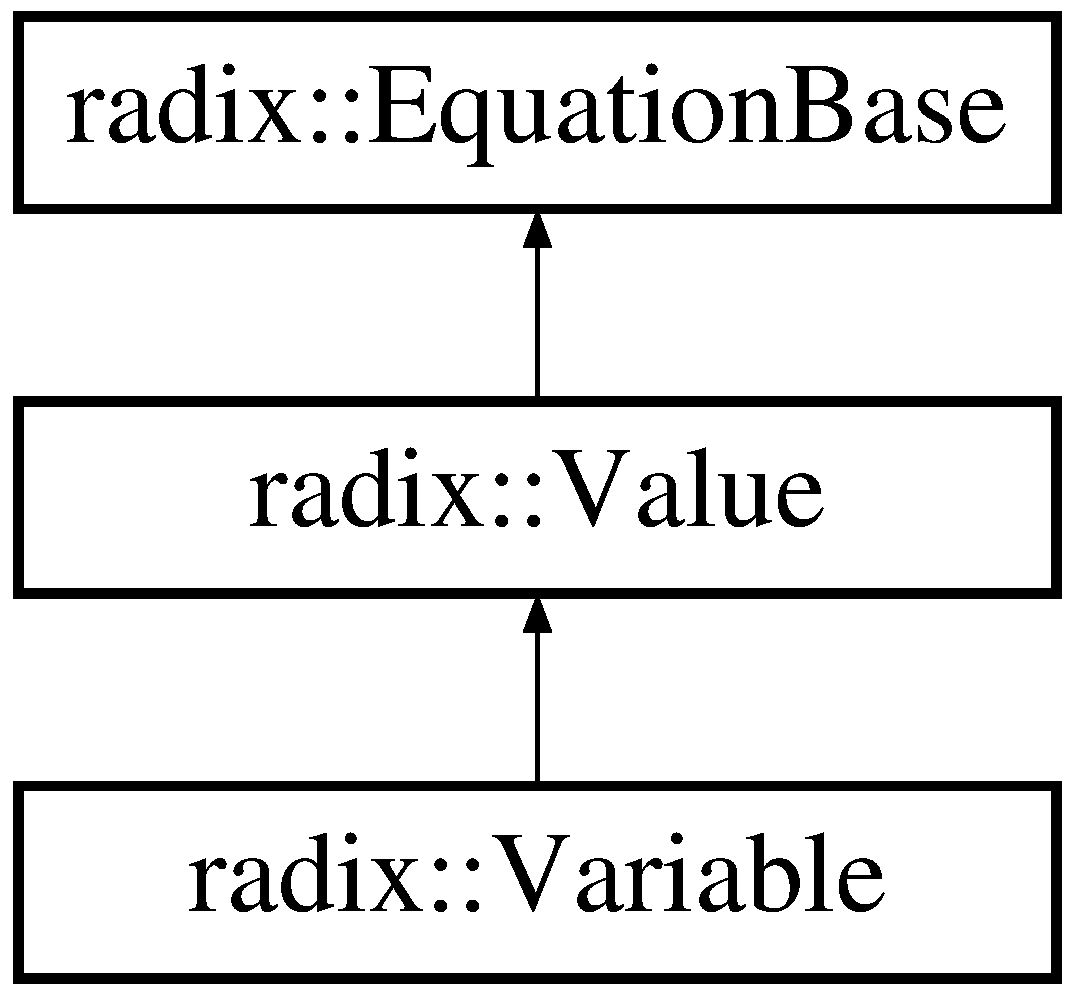
\includegraphics[height=3.000000cm]{classradix_1_1Variable}
\end{center}
\end{figure}
\subsection*{Public Member Functions}
\begin{DoxyCompactItemize}
\item 
\mbox{\Hypertarget{classradix_1_1Variable_afda152d664203a2e660dcec4e7f4f6ee}\label{classradix_1_1Variable_afda152d664203a2e660dcec4e7f4f6ee}} 
{\bfseries Variable} (const std\+::string \&ref\+\_\+str)
\item 
\mbox{\Hypertarget{classradix_1_1Variable_ad74660a33f619558be499c0c87d71e73}\label{classradix_1_1Variable_ad74660a33f619558be499c0c87d71e73}} 
{\bfseries Variable} (const char \&ref\+\_\+ch)
\item 
\mbox{\Hypertarget{classradix_1_1Variable_aac2a333d710dae5a8a1499019e6b0541}\label{classradix_1_1Variable_aac2a333d710dae5a8a1499019e6b0541}} 
void {\bfseries Set\+Ref} (const std\+::string \&ref\+\_\+str)
\item 
\mbox{\Hypertarget{classradix_1_1Variable_aa56b21d16749be50b78eea83b77d1700}\label{classradix_1_1Variable_aa56b21d16749be50b78eea83b77d1700}} 
void {\bfseries Set\+Ref} (const char \&ref\+\_\+ch)
\item 
\mbox{\Hypertarget{classradix_1_1Variable_a072e338af8cc3833a18a8648de46c7c7}\label{classradix_1_1Variable_a072e338af8cc3833a18a8648de46c7c7}} 
void {\bfseries Set\+Val} (std\+::shared\+\_\+ptr$<$ \hyperlink{classradix_1_1Value}{Value} $>$ val)
\item 
\mbox{\Hypertarget{classradix_1_1Variable_a66ba56c31e8d4bc795f83e13c236c5ba}\label{classradix_1_1Variable_a66ba56c31e8d4bc795f83e13c236c5ba}} 
std\+::string {\bfseries Get\+Ref} () const
\item 
\mbox{\Hypertarget{classradix_1_1Variable_a2f282cab8f47b1fac30df8f7df3f8acd}\label{classradix_1_1Variable_a2f282cab8f47b1fac30df8f7df3f8acd}} 
std\+::shared\+\_\+ptr$<$ \hyperlink{classradix_1_1Value}{Value} $>$ {\bfseries Get\+Val} () const
\item 
\mbox{\Hypertarget{classradix_1_1Variable_a336d28b81443a656d72c713f4fa73c63}\label{classradix_1_1Variable_a336d28b81443a656d72c713f4fa73c63}} 
std\+::string {\bfseries Latex} () const
\item 
\mbox{\Hypertarget{classradix_1_1Variable_a46f38d8ae307f2e7846b76f15b727201}\label{classradix_1_1Variable_a46f38d8ae307f2e7846b76f15b727201}} 
\hyperlink{classradix_1_1Variable}{Variable} \& {\bfseries operator=} (const std\+::shared\+\_\+ptr$<$ \hyperlink{classradix_1_1Value}{Value} $>$ val)
\item 
\mbox{\Hypertarget{classradix_1_1Variable_aa13e5f5df26da89d3b8984061ca38bd8}\label{classradix_1_1Variable_aa13e5f5df26da89d3b8984061ca38bd8}} 
{\bfseries operator std\+::shared\+\_\+ptr$<$ Value $>$} ()
\item 
\mbox{\Hypertarget{classradix_1_1Variable_afcb88f325eaf93a53c6c55186e823925}\label{classradix_1_1Variable_afcb88f325eaf93a53c6c55186e823925}} 
{\bfseries operator std\+::shared\+\_\+ptr$<$ Equation\+Base $>$} ()
\end{DoxyCompactItemize}
\subsection*{Additional Inherited Members}


The documentation for this class was generated from the following files\+:\begin{DoxyCompactItemize}
\item 
include/value/variable.\+hpp\item 
source/value/variable.\+cpp\end{DoxyCompactItemize}

%--- End generated contents ---

% Index
\backmatter
\newpage
\phantomsection
\clearemptydoublepage
\addcontentsline{toc}{chapter}{Index}
\printindex

\end{document}
